\begin{refsection}[research/tama/group.bib]
\nocite{*}
\chapter{Computational Structural Biology Research Unit}

\section{Members}

\begin{itemize}
  \item[] Florence Tama (Unit Leader)
  \item[] Atsushi Tokuhisa  (Research Scientist)
  \item[] Miki Nakano (Post-doctoral researcher)
  \item[]  Sandhya Tiwari (Post-doctoral researcher)
  \item[]  Sachiko Kikumoto (Assistant)
  \item[]  Yumeno Kusahara (Assistant)
\end{itemize}

\section{Research Activities}
Biological molecular complexes such as proteins and RNAs are of great interest in the area of molecular biology as they are involved in cell replication, gene transcription, protein synthesis, regulation of cellular transport and other core biological functions. Those systems undergo large conformational transitions to achieve functional processes. Therefore characterization of structures of these macromolecular complexes is crucial to understand their functional mechanisms, and play an important role in the development of new drugs to treat human disease.  

Experimentally, X-ray crystallography has been the primary tool to study protein conformations,� providing high-resolution structures. Cryo electron microscopy (EM) has provided, although at lower-resolution, critical information on structure and dynamics of large biological molecules. More recently, efforts like in Riken/SPring 8 have focused on developing intense X-ray free-electron laser (XFEL) light sources, which offer a new possibility to image single biological macromolecules. Since crystallization is not necessary for such a protein structure analysis, it would be possible to investigate the structure of macromolecular complexes and proteins under various physiological conditions or to observe elementary steps of a biochemical function. However, at the current experimental condition, it cannot achieve atomic level resolution such as obtained by X-ray crystallography.

Computationally, methods have been developed to predict structures from low-resolution data such as cryo-EM either using rigid body fitting or flexible deformations of known atomic structures. In addition, even when structures of the molecules are unknown, atomic models can be predicted using homology modeling and ab initio predictions. While ab initio prediction still remains difficult for large proteins, success in predicting small proteins have been observed. Finally, algorithms to analyze protein/proteins interactions also have shown success in predicting proteins complexes.

Our research focuses on the development of computational tools to study biological systems, more specifically to help in their 3D structural determination using various experimental techniques and to analyze their potential interactions with small molecules in order to design new drugs. The ultimate line of our interdisciplinary research is too bring experimental data as obtained from X-ray, cryo-EM and XFEL with development and applications of computational tools through the K computer to acquire knowledge on the structure of a physiologically important protein complexes that are unattainable with existing experimental techniques, and to contribute to development of drug design and medical treatment in collaboration with pharmaceutical companies. 


\section{Research Results and Achievements}
\subsection{Refinement 2D raw data}

Following discussions with experimental groups, in this fiscal year, we have been working on refinement of real 2D data. Diffraction patterns from X-ray Free Electron Laser is approximately the Fourier transform of 2D projection image of the target, however the detectors can observe only the intensity and phase cannot be determined. Reconstruction of 2D projection images requires the phase, and a common approach is "phase reconstruction", in which numerical algorithm is used to estimate the phase. To further improve agreement (R-factor) with experimental data, we developed a method that utilizes Limited memory Broyden Fletcher Goldfarb Shanno B Nonlinear Optimizer and Basinhopping algorithm. Such refinement will allow for a more accurate interpretation of the real 2D data derived from XFEL experiments  (see Figure \localref{fig:sample-label1})

\begin{figure}
\centering
  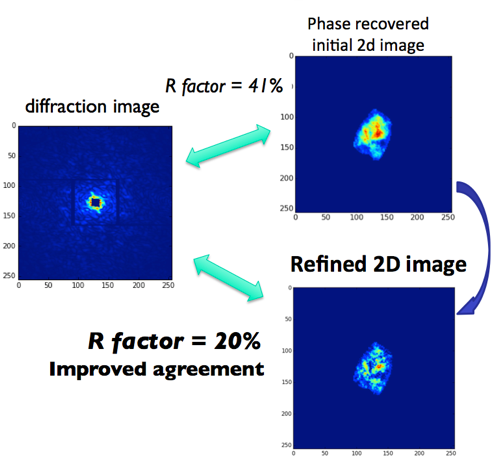
\includegraphics[width=0.5\textwidth,keepaspectratio,natwidth=193,natheight=40]
  {research/tama/Figures/picture1.png}
  \caption{Refinement of 2D raw data}
  \locallabel{fig:sample-label1}
\end{figure}

\subsection{3D reconstruction from XFEL data}
In order to restore the 3D real structure of the molecule from the diffraction patterns obtained by XFEL experiments, computational algorithms are necessary as one needs to estimate the laser beam incidence angles to the molecule and retrieve the phase information. We are developing a program package for XFEL analysis based on XMIPP, which is commonly used for image processing of single-particle 3D cryo electron microscopy. Since XMIPP is designed to work with 2D data in real space, some of the routine were modified to deal with 2D diffraction data in Fourier space. The overall protocol used for 3D reconstruction is shown in Figure \localref{fig:sample-label2}.

\begin{figure}
\centering
  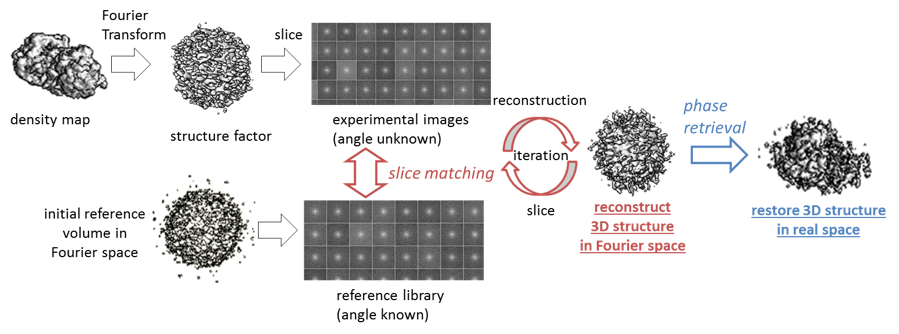
\includegraphics[width=1\textwidth,keepaspectratio,natwidth=386,natheight=80]
  {research/tama/Figures/picture2.png}
  \caption{3D reconstruction from XFEL}
  \locallabel{fig:sample-label2}
\end{figure}


The protocol was tested using simulated diffraction images from the crystal structure of a translation termination complex formed by the Thermus thermophilus 70S ribosome bound with release factor RF2 (PDB ID = 4V67). The algorithm is able to estimate relative orientations of the diffraction images. The resulting reconstructed 3D structure is shown in Figure \localref{fig:sample-label3}.

\begin{figure}
\centering
  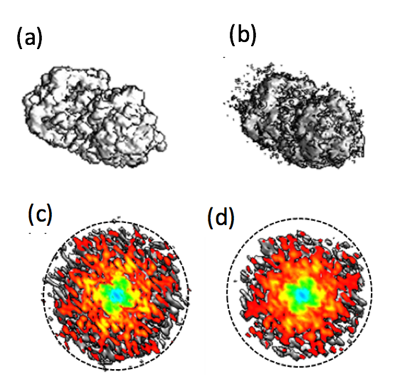
\includegraphics[width=0.5\textwidth,keepaspectratio,natwidth=193,natheight=40]
  {research/tama/Figures/picture3.png}
  \caption{3D XFEL reconstruction for the ribosome. (a) Electron density map of the ribosome created from the X-ray structure. (b) Electron density map obtained using the protocol described in Fig \localref{fig:sample-label2}. (c) and (d) are cross section views of the structure factor (structure in Fourier space) for (a) and (b) respectively}
  \locallabel{fig:sample-label3}
\end{figure}

\subsection{Fast image filtering procedure}

For current XFEL experiments, the number of diffraction data is limited. Therefore, we have been developing new approaches to obtain structural and dynamical information by combining such low-resolution and limited information from XFEL data with other data, such as X-ray structure and computational tools. We published algorithms to identify a conformation, among several candidates, that agrees with XFEL data.

To perform ab initio modeling, a large number of conformations need to be explored to find a good model that agrees with the data. Thus it is important that the agreement between the models and the target diffraction can be evaluated quickly. In our previous study, diffraction patterns were first simulated from the candidate models, and then the simulated diffraction patterns were compared with the target pattern. While this approach is accurate, it is also time consuming; the simulation of X-ray diffractions is mathematically complex and 2D image comparisons need to be performed for different alignment angles.

To speed up this process, we have been developing an algorithm to filter out unpromising models using information reduction technique. In this approach, from the original 2D target image, 1D radial profile (average over circles) is calculated. Then for each model, corresponding 1D profile is calculated and compared against the target 1D profile. Such 1D profile can be quickly calculated directly from mass distribution, and 1D profile comparison is also fast. Since 1D approach is an approximation, this is used as a preliminary filtering process to reject the models with low 1D score. Then, we evaluate more precise similar score for the remaining models using 2D images to select the best models.
Recently, we developed a new equation that can increase the sensitivity of the filtering:

\begin{equation}
\tilde{I}(q)��= \int^\infty_0 p(s) J_0(2\pi qs) ds��\label{relation}
\end{equation}
where $I(q)$ is the 2D profile used for comparison, $J$ is a Bessel function, and $p(s)$ is 2D distance distribution function. This new formula replaces conventional Debye equation used for SAXS analysis and more accurate for 2D diffraction image analysis such as used here. We have tested this approach for a biological molecule to confirm the validity of this formalism (see Figure  \localref{fig:sample-label4})

\begin{figure}
\centering
  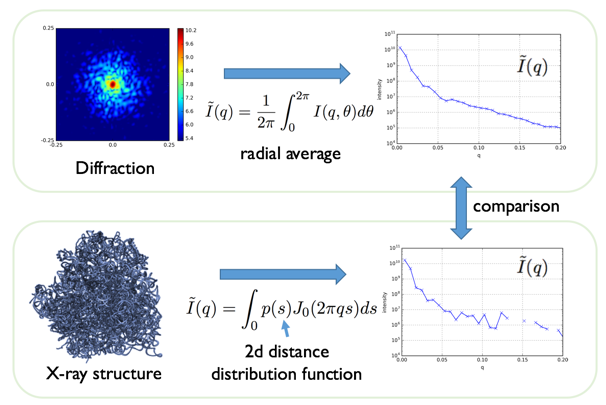
\includegraphics[width=0.7\textwidth,keepaspectratio,natwidth=193,natheight=40]
  {research/tama/Figures/picture4.png}
  \caption{Fast image filtering procedure}
  \locallabel{fig:sample-label4}
\end{figure}


\subsection{DNA solvation properties}

Under physiological conditions, where various biomolecules and other components are present, DNA strands may adopt many different structures in addition to the canonical B-form duplex. Such effects of molecular crowding on thermal stabilities of DNA structures maybe associated with the properties of the water molecules around the DNAs. 

Using MD simulations, we studied the thermodynamic properties of water molecules around a hairpin duplex and a G-quadruplex to understand how cosolutes affect the thermal stability of DNA structures. Our findings suggest that differences in the hydration shell structure around DNAs are one factor that affects the thermal stabilities of DNA structures under the crowding conditions. In addition, thermodynamic properties of water molecules around single- and double-stranded DNAs were investigated. Upon the formation of double-stranded DNA, thermodynamics features of the water molecules is primarily changed in the minor groove. Free energies of water molecules around double-stranded DNA are lower than those around single-stranded DNA even in the second and third hydration shells

\begin{figure}
\centering
  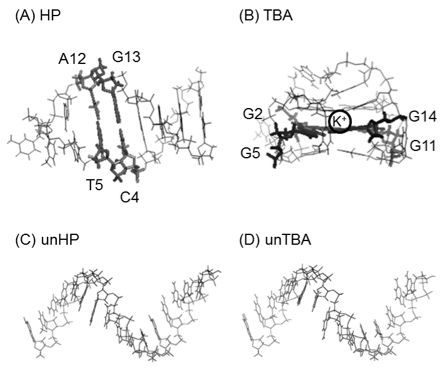
\includegraphics[width=0.7\textwidth,keepaspectratio,natwidth=193,natheight=40]
  {research/tama/Figures/picture5.png}
  \caption{Different forms of DNA}
  \locallabel{fig:sample-label5}
\end{figure}




\section{Schedule and Future Plan}

We are planning to continue to develop tools to analyze XFEL data to obtain structural information of biological molecules. In particular, we intend to improve the 3D reconstruction protocol proposed for XFEL data by providing more informed initial reference volume. To achieve such a goal, we plan to maintain a database of shapes and associated diffraction patterns found in biological molecules. In addition, efficiency of the protocols in terms of speed will be addressed. We will also apply our tools to experimental data. In parallel, we will continue the development of algorithms to extract information from a limited number of low-resolution data, since only limited experiments might be feasible for some systems even with the development of experimental techniques. Ab-initio modeling of sample shapes based on the use of simplified representations of the biological molecules as well as optimization procedure will be further developed taking advantage of the newly fast filtering scheme.

As experimental data from cryo-EM and for XFEL will continue to grow in numbers, analysis of such big dataset will increase the necessity of high performance computing. We aim to utilize K and post-K to break the limitation of current processing power to obtain new level of structural information of biological complexes from EM and XFEL data. For this goal, we plan to develop softwares to analyze data to obtain structural models that can utilize computers in different sizes such as cluster and supercomputer. By sharing the software and results from structural modeling with other research institutes, we aim to contribute to the structural biology community.

As our research focuses on developing computational tools to analyze low-resolution experimental data, we intend to establish collaborations with experimental groups in Japan and abroad in order to study structure, function and dynamics of biological molecules.

%%% DO NOT EDIT BELOW

\section{Publications}

%\printbibliography[keyword=journal, heading=subbibliography, title={Journal Articles}, prefixnumbers={1-}, resetnumbers=true]
%\printbibliography[keyword=proceedings, heading=subbibliography, title={Conference Papers}, prefixnumbers={2-}, resetnumbers=true]
%\printbibliography[keyword=invited, heading=subbibliography, title={Invited Talks}, prefixnumbers={3-}, resetnumbers=true]
%\printbibliography[keyword=poster, heading=subbibliography, title={Posters and Presentations}, prefixnumbers={4-}, resetnumbers=true]
%\printbibliography[keyword=deliverable, heading=subbibliography, title={Patents and Deliverables}, prefixnumbers={5-}, resetnumbers=true]

\printbibliography[keyword=journal, heading=subbibliography, title={Journal Articles}, resetnumbers=true]
\printbibliography[keyword=proceedings, heading=subbibliography, title={Conference Papers}]
\printbibliography[keyword=invited, heading=subbibliography, title={Invited Talks}]
\printbibliography[keyword=poster, heading=subbibliography, title={Posters and Presentations}]
\printbibliography[keyword=deliverable, heading=subbibliography, title={Patents and Deliverables}]

\end{refsection}
